\chapter{API}
\label{sec:module.API}

Unsere AITools \gls{API} dient als Grundbaustein aller \gls{AI} Komponenten, entkapselt die Interfaces zu unseren \gls{AI} Modulen und bietet den \gls{AI} Modulen sowie dem Ants Package die Basisklassen an, welche �berall verwendet werden (s.a. Abbildung \ref{fig:modulesOverview}). Der Inhalt ist wie folgt:

\section{Entities}
\label{sec:mocule.API.Entities}

Das Package Entities beinhaltet die Klassen, die von den Such- und Strategiealgorithmen sowie vom \gls{Bot} verwendet werden.

\begin{figure}[H]
\centering
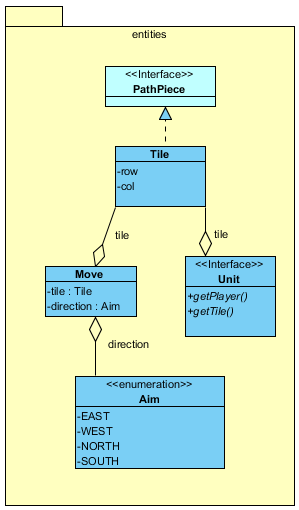
\includegraphics[width=0.4\textwidth]{91_bilder/apiEntities}
\caption{Entities}
\label{fig:apiEntities}
\end{figure}

\begin{itemize}
\item
\textbf{Aim}: Richtungsangabe zum Beschreiben einer Bewegung der Ameise. Da sich die Ameisen nur geradeaus bewegen k�nnen, beschr�nken sich die g�ltigen Werte auf die vier Himmelsrichtungen.
\item
\textbf{\gls{Tile}}: Repr�sentiert eine Zelle auf dem Spielfeld, welche mit Row (Zeile) und Column (Spalte) definiert ist. Die Klasse Tile implementiert das PathPiece Interface (s. Abschnitt \ref{sec:module.API.Search})
\item
\textbf{Move}: Diese Klasse beschreibt einen Spielzug mit den Eigenschaften \gls{Tile}, von wo aus der Zug statt findet, und Aim, in welche Richtung der Zug ausgef�hrt wird.
\item
\textbf{Unit}: Unit besteht aus \gls{Tile} und Spieler und definiert eine Einheit eines Spielers auf der Karte.
\end{itemize}

\section{Map}
\label{sec:mocule.API.Map}

Im Map-Package sind verschiedene Karten-Typen definiert, die die Interaktion mit der Spielwelt erm�glichen.

\begin{figure}[H]
\centering
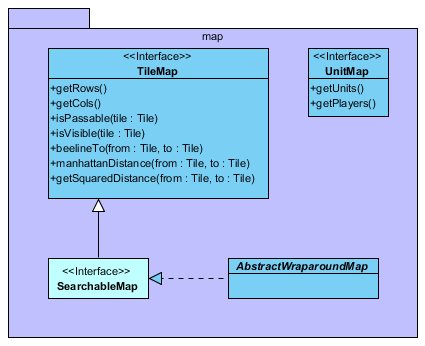
\includegraphics[width=0.7\textwidth]{91_bilder/apiMap}
\caption{Map API}
\label{fig:apiMap}
\end{figure}

\begin{itemize}
\item
\textbf{TileMap}:  Dieses Interface definiert, welche Methoden eine auf \gls{Tile}s aufbauende Spielkarte anbieten muss. Dazu geh�ren die Masse der Karte, die Gel�ndebeschaffenheit, also ob eine Zelle f�r den Spieler sichtbar und passierbar ist, sowie Distanz-Messfunktionen wie ManhattanDistance, Luftlinie, quadrierte Distanz.
\item
\textbf{UnitMap}:  Dieses Interface definiert, welche Methoden eine Spielkarte implementieren muss, um Zugriff auf die in der Karte platzierten Einheiten zu bieten. Die Methode \texttt{getPlayers()} gibt eine Liste der Spieler zur�ck, die Einheiten auf der Karte kontrollieren, die Methode \texttt{getUnits()} gibt alle bekannten Einheiten zur�ck.
\item
\textbf{AbstractWraparoundMap}: Implementiert das Interface SearchableMap (s. \ref{sec:module.API.Search}). Hier sind alle Methoden implementiert, welche die Karte anbieten muss, damit sie mit den Suchalgorithmen verwendet werden kann. Zudem sind einige der vordefinierten Methoden aus TileMap implementiert.
\item
\textbf{WorldType}: WorldType ist ein Enum und definiert die Art der Karte. Der Typ \texttt{Globus} hat keine Kartenr�nder, ist also ringsum begehbar. Von diesem Typ ist auch die AbstractWraparoundMap Klasse, welche als Basisklasse unserer World-Karte\footnote{s. Kapitel 
\ref{sec:module.Ants.State.World}} dient. Folglich sind auch die Karten  der Ants Challenge ''WrapAround``-Karten. Der zweite Enumtyp ist \texttt{Pizza} und definiert eine Welt wie man sich unsere Erde vor 500 Jahren noch vorstellte, eine Scheibe mit R�ndern, welche die Welt begrenzen. Dieser zweite Typ wurde provisorisch erstellt. Falls unsere \gls{API} eine Weiterverwendung findet, kann dieser Typ zus�tzlich implementiert werden.
\end{itemize}


\section{Search}
\label{sec:module.API.Search}

Search beinhaltet alle Basisklassen und -interfaces der Suche.

\begin{figure}[H]
\centering
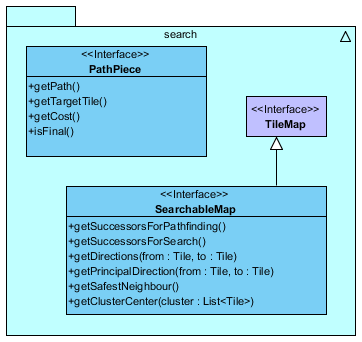
\includegraphics[width=0.6\textwidth]{91_bilder/apiSearch}
\caption{Search API}
\label{fig:apiSearch}
\end{figure}

\begin{itemize}
\item
\textbf{PathPiece}: Das PathPiece ist ein Interface f�r Strukturen, die als Suchknoten in der Pfadsuche verwendet werden k�nnen. Implementierende Klassen sind Edge (rep�sentiert eine Kante in einem Cluster) und \gls{Tile}. Erweiterungen dieser Klassen sind DirectedEdge (gerichtete Kanten) und Vertex (ein Knoten mit anliegenden Kanten).
\item
\textbf{SearchableMap}: Das Interface SearchableMap erweitert das Interface TileMap. Es beschreibt die Methoden zur Pfadsuche, wie \texttt{getSuccessors()}, \texttt{getCost()}, oder \texttt{getPath()}. Die Unterscheidung zwischen \texttt{getSuccessorsForPathfinding()} und \texttt{getSuccessorsForSearch()} haben wir eingef�hrt, damit bei der Pfadsuche bestimmte \gls{Tile}s von vornherein ausgeschlossen werden k�nnen. (Konkret haben wir so verhindert, dass Pfade �ber unsere eigenen H�gel f�hren.)
\end{itemize}

\section{Strategy}
\label{sec:mocule.API.Strategy}

In diesem Package befinden sich die Karteninterfaces, welche f�r das Anwenden von Strategie und Taktikalgorithmen grundlegend sind.

\begin{figure}[H]
\centering
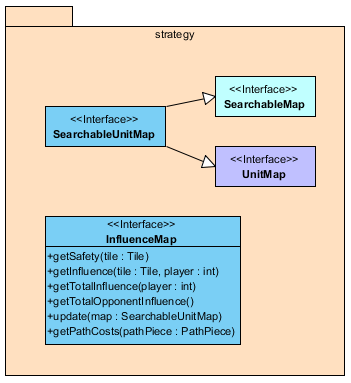
\includegraphics[width=0.6\textwidth]{91_bilder/apiStrategy}
\caption{Strategy API}
\label{fig:apiStrategy}
\end{figure}

\begin{itemize}
\item
\textbf{SearchableUnitMap}: Dieses Interface dient ausschliesslich zur Zusammenf�hrung der beiden Interfaces UnitMap und SearchableMap.
\item
\textbf{InfluenceMap}: Dieses Interface definiert Methoden, die eine \gls{InfluenceMap} anbieten muss. So muss sie f�r ein bestimmtes Tile und einen bestimmten Spieler den Einfluss angeben k�nnen, oder sie muss Auskunft �ber die Sicherheit eines bestimmten \gls{Tile}s geben k�nnen. Mit der \texttt{update()} Methode kann die InfluenceMap aktualisiert werden.
\end{itemize}